\documentclass[a4paper,12pt]{report}

\usepackage[utf8x]{inputenc}
\usepackage[T2A]{fontenc}
\usepackage[english, russian]{babel}

% Опционно, требует  apt-get install scalable-cyrfonts.*
% и удаления одной строчки в cyrtimes.sty
% Сточку не удалять!
% \usepackage{cyrtimes}

% Картнки и tikz
\usepackage{graphicx}
\usepackage{tikz}
\usetikzlibrary{snakes,arrows,shapes}


% Увы, поля придётся уменьшить из-за листингов.
\topmargin -1cm
\oddsidemargin -0.5cm
\evensidemargin -0.5cm
\textwidth 17cm
\textheight 24cm

\sloppy



% Оглавление в PDF
\usepackage[
bookmarks=true,
colorlinks=true, linkcolor=black, anchorcolor=black, citecolor=black, menucolor=black,filecolor=black, urlcolor=black,
unicode=true
]{hyperref}

% Для исходного кода в тексте
% \newcommand{\Code}[1]{\texttt{#1}}

% Некоторая русификация.
% \usepackage{misccorr} % Oh shi^W^W, оно не работает с report.
\usepackage{indentfirst}
\renewcommand{\labelitemi}{\normalfont\bfseries{--}}

% На дворе XXI век, но пакет listings всё ещё не пашет с русскими комментариями!

% Пакет listings для простой вставки исходников
% \usepackage{listings}
% Параметры оформления
% \lstset{
% showspaces=false,
% showtabs=false,
% frame=single,
% tabsize=4,
% basicstyle=\ttfamily,
% identifierstyle=\ttfamily,
% commentstyle=\itshape,
% stringstyle=\ttfamily,
% keywordstyle=\ttfamily,
% breaklines=true
% }
% Русский в комментариях.
% \lstset{escapebegin=\begin{cyr},escapeend=\end{cyr}}



% А это взято из файла, сгенерённого doxygen
\usepackage{calc}
\usepackage{array}
\newenvironment{Code}
{\footnotesize}
{\normalsize}
\newcommand{\doxyref}[3]{\textbf{#1} (\textnormal{#2}\,\pageref{#3})}
\newenvironment{DocInclude}
{\footnotesize}
{\normalsize}
\newenvironment{VerbInclude}
{\footnotesize}
{\normalsize}
\newenvironment{Image}
{\begin{figure}[H]}
{\end{figure}}
\newenvironment{ImageNoCaption}{}{}
\newenvironment{CompactList}
{\begin{list}{}{
  \setlength{\leftmargin}{0.5cm}
  \setlength{\itemsep}{0pt}
  \setlength{\parsep}{0pt}
  \setlength{\topsep}{0pt}
  \renewcommand{\makelabel}{\hfill}}}
{\end{list}}
\newenvironment{CompactItemize}
{
  \begin{itemize}
  \setlength{\itemsep}{-3pt}
  \setlength{\parsep}{0pt}
  \setlength{\topsep}{0pt}
  \setlength{\partopsep}{0pt}
}
{\end{itemize}}
\newcommand{\PBS}[1]{\let\temp=\\#1\let\\=\temp}
\newlength{\tmplength}
\newenvironment{TabularC}[1]
{
\setlength{\tmplength}
     {\linewidth/(#1)-\tabcolsep*2-\arrayrulewidth*(#1+1)/(#1)}
      \par\begin{tabular*}{\linewidth}
             {*{#1}{|>{\PBS\raggedright\hspace{0pt}}p{\the\tmplength}}|}
}
{\end{tabular*}\par}
\newcommand{\entrylabel}[1]{
   {\parbox[b]{\labelwidth-4pt}{\makebox[0pt][l]{\textbf{#1}}\vspace{1.5\baselineskip}}}}
\newenvironment{Desc}
{\begin{list}{}
  {
    \settowidth{\labelwidth}{40pt}
    \setlength{\leftmargin}{\labelwidth}
    \setlength{\parsep}{0pt}
    \setlength{\itemsep}{-4pt}
    \renewcommand{\makelabel}{\entrylabel}
  }
}
{\end{list}}
\newenvironment{Indent}
  {\begin{list}{}{\setlength{\leftmargin}{0.5cm}}
      \item[]\ignorespaces}
  {\unskip\end{list}}


\begin{document}

\tableofcontents
\setcounter{page}{3} % начать нумерацию с номера три
\addcontentsline{toc}{chapter}{Введение}
\chapter*{Введение}
\subsection{Цели и задачи}

Цель: 
    Разработать \textbf{SMTP-сервер} используя вызов select и рабочие процессы. Журналирование
    в отдельном процессе.

Задачи:
\begin{itemize}
    \item Проанализировать архитектурное решение
    \item Разработать подход для обработки входящих соединений и хранения входящих писем в maildir
    \item Рассмотреть \textbf{SMTP}-протокол
    \item Реализовать программу для получения писем по протоколу \textbf{SMTP}
    \item Реализовать метод журналирования в отдельном процессе\textbf{SMTP}
\end{itemize}

\chapter{Аналитический раздел}

\section*{Предметная область}
Согласно обозначенному протоколу в рамках данной работы, в системе устанавливаются отношения "отправитель - получатель", причем отправитель может отправить письмо нескольким получателям. Основная единица данных, передаваемая по протоколу - письмо, которое включает в себя отправителя и получателя, причем получателей может быть несколько. Также письмо содержит в себе единственное тело, которое может быть использовано как для последующей передачи, так и для хранения на сервере.
Таким образом, в рамках предметной области можно выделить 3 вида сущностей:
\begin{itemize}
    \item 1. Сервер
    \item 2. Клиент
    \item 3. Письмо
\end{itemize}
\section*{Сервер}
\subsection*{Преимущества и недостатки условия задачи}
Согласно условию задачи, в работе сервера предлагается исполльзовать многопроцессную систему. Данная архитектура имеет следующие преимущества:
\begin{itemize}
    \item 1. Простота разработки. Фактически, мы запускаем много копий однопоточного приложения и они работают независимо друг от друга. Можно не использовать никаких специфически многопоточных API и средств межпроцессного взаимодействия.
    \item 2. Высокая надежность. Аварийное завершение любого из процессов никак не затрагивает остальные процессы.
    \item 3. Хорошая переносимость. Приложение будет работать налюбой многозадачной ОС
    \item 4. Высокая безопасность. Разные процессы приложения могут запускаться от имени разных пользователей. Таким образом можно реализовать принцип минимальных привилегий, когда каждый из процессов имеет лишь те права, которые необходимы ему для работы. Даже если в каком-то из процессов будет обнаружена ошибка, допускающая удаленное исполнение кода, взломщик сможет получить лишь уровень доступа, с которым исполнялся этот процесс.
\end{itemize}
При этом данная архитектура имеет следующие недостатки:
\begin{itemize}
    \item 1. Далеко не все прикладные задачи можно предоставлять таким образом. Например, эта архитектура годится для сервера, занимающегося раздачей статических HTMLстраниц, но совсем непригодна для сервера баз данных и многих серверов приложений.
    \item 2. Создание и уничтожение процессов – дорогая операция, поэтому для многих задач такая архитектура неоптимальна.
\end{itemize}
Поэтому для минимизации операций создания и уничтожения процессов предлагается архитектурное решение, представляющее собой пул процессов,
создаанных заранее. Это позволит фиксировать число операций создания процесса. При этом слушающие сокеты сервера должны наследоваться каждым создаваемым процессом. Это делается для решения проблемы распределения соединений между процессами одной группы. 
\chapter{Конструкторский раздел}

\section{Конечный автомат состояний сервера}

Конечный автомат состояний сервера представлен на Рис.~\ref{fig:server_fsm} 

\begin{figure}
	\centering
	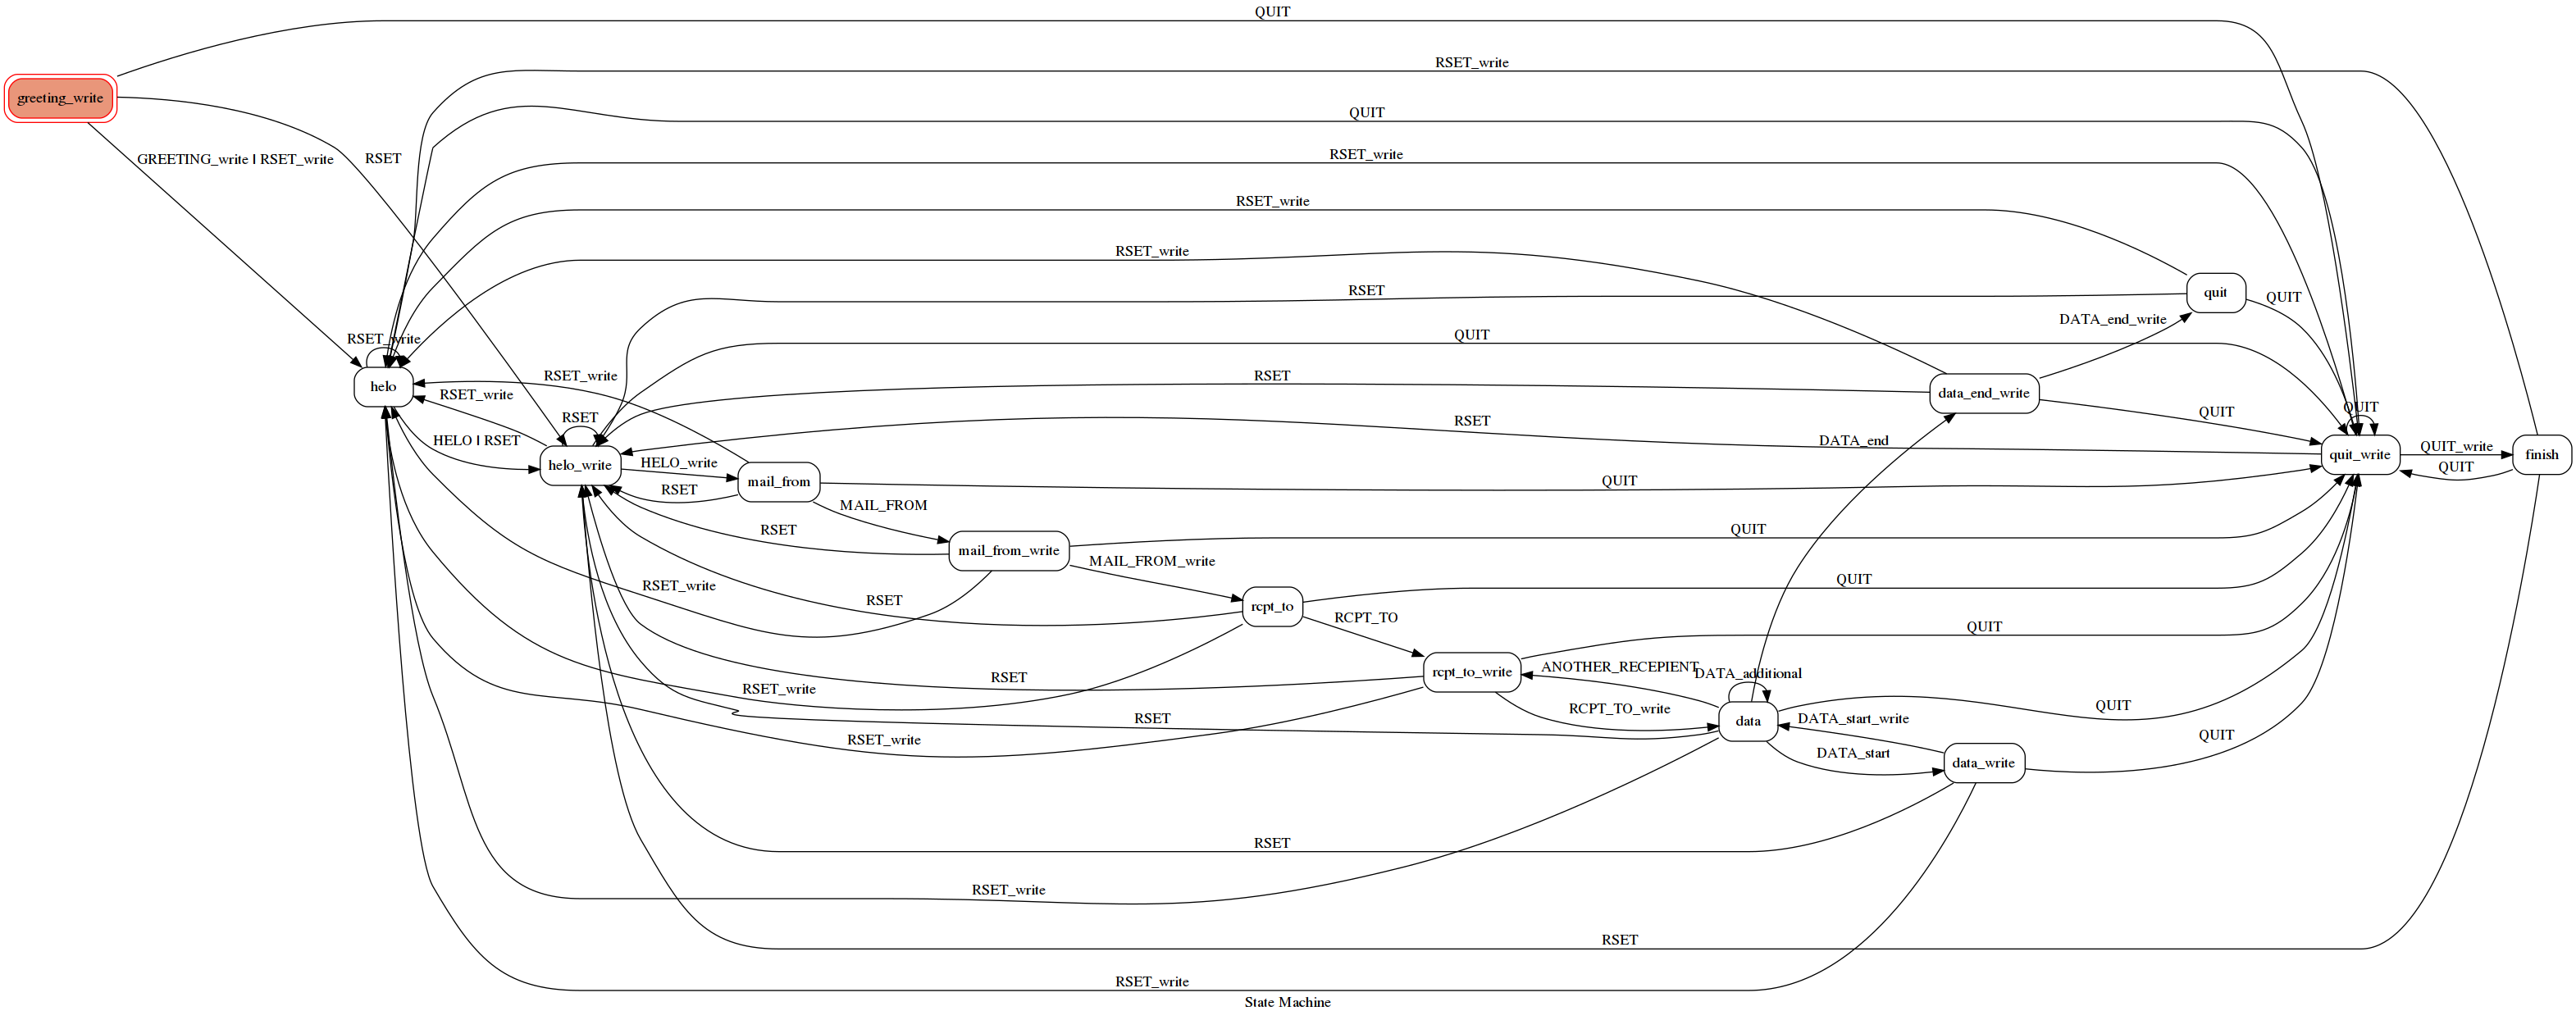
\includegraphics[width=\textwidth]{static/server_dot.png}
	\caption{Состояния сервера}
	\label{fig:server_fsm}
\end{figure}

\subsection{Синтаксис команд протокола}
Ниже приведен формат команд сообщений протокола в виде регулярных выражений
\begin{enumerate}
\item \textbf{EHLO}: {\it EHLO [w+]+\/}
\item \textbf{HELO}: {\it HЕLO [w+]+\/}
\item \textbf{MAIL}: {\it MAIL FROM <[\textbackslash w]+@[\textbackslash w]+\.[\textbackslash w]+>\/}
\item \textbf{RCPT}: {\it RCPT <[\textbackslash w]+@[\textbackslash w]+\.[\textbackslash w]+>\/}
\item \textbf{DATA}: {\it DATA\/}
\item \textbf{RSET}: {\it RSET\/}
\item \textbf{QUIT}: {\it QUIT\/}
\end{enumerate}

\subsection*{Представление данных}
Ниже приведена диаграмма представления данных в системе
\begin{figure}
\centering
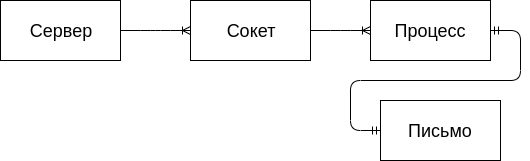
\includegraphics[width=\textwidth]{static/physical.png}
\caption{Физическая диаграмма сущностей}
\label{fig:phys_diagram}
\end{figure}


\subsection{Алгоритм обработки соединений}
\begin{verbatim}


 ПОКА (процесс_работает == 1) 
      Добавить дескрипторы слушающих сокетов в сет читателей 
      Добавить дескрипторы клиентских сокетов в сет читателей 
      Ожидать соединения на одном из сокетов (время = 5с) 
      ЕСЛИ есть запрос ТО 
        ДЛЯ каждого слушающего сокета 
           ЕСЛИ действие на одном из слушающих сокетов ТО 
               Принять новое соединение 
               Инициализировать новый сокет 
           КОНЕЦ ЕСЛИ 
           ЕСЛИ действие на одном из клиентских сокетов ТО 
           		Обработать действие в соответствии с протоколом 
           КОНЕЦ ЕСЛИ 
        КОНЕЦ ДЛЯ 
        ДЛЯ каждого сокета записи
           ЕСЛИ действие на одном из клиентских сокетов ТО 
              Обработать действие в соответствии с протоколом 
           КОНЕЦ ЕСЛИ 
        КОНЕЦ ДЛЯ 
      КОНЕЦ ЕСЛИ 
 КОНЕЦ ПОКА 

\end{verbatim}

\chapter{Технологический раздел}

\section{Сборка программы}

Сборка программы описана в файле \textit{Makefile} системы сборки \textit{make}. Рис.~\ref{fig:make}. Изображение с конечным автоматом генерируется срествами библиотеки transitions.

\begin{figure}
\centering
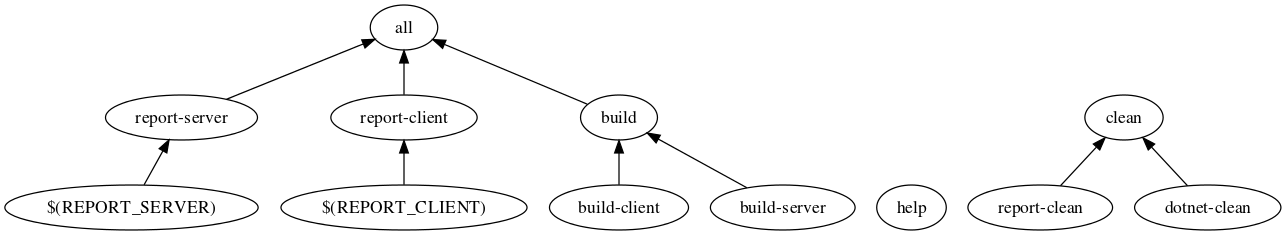
\includegraphics[width=\textwidth]{include/make.png}
\caption{Сборка программы}
\label{fig:make}
\end{figure}

\section{Графы вызова функций}

Поскольку функций много, графы вызовов разбиты на два рисунка. На рис.~\ref{fig:cflow01} показаны основные функции, на рис.~\ref{fig:cflow02}~-- функции обработки команд. 

\begin{figure}
\centering
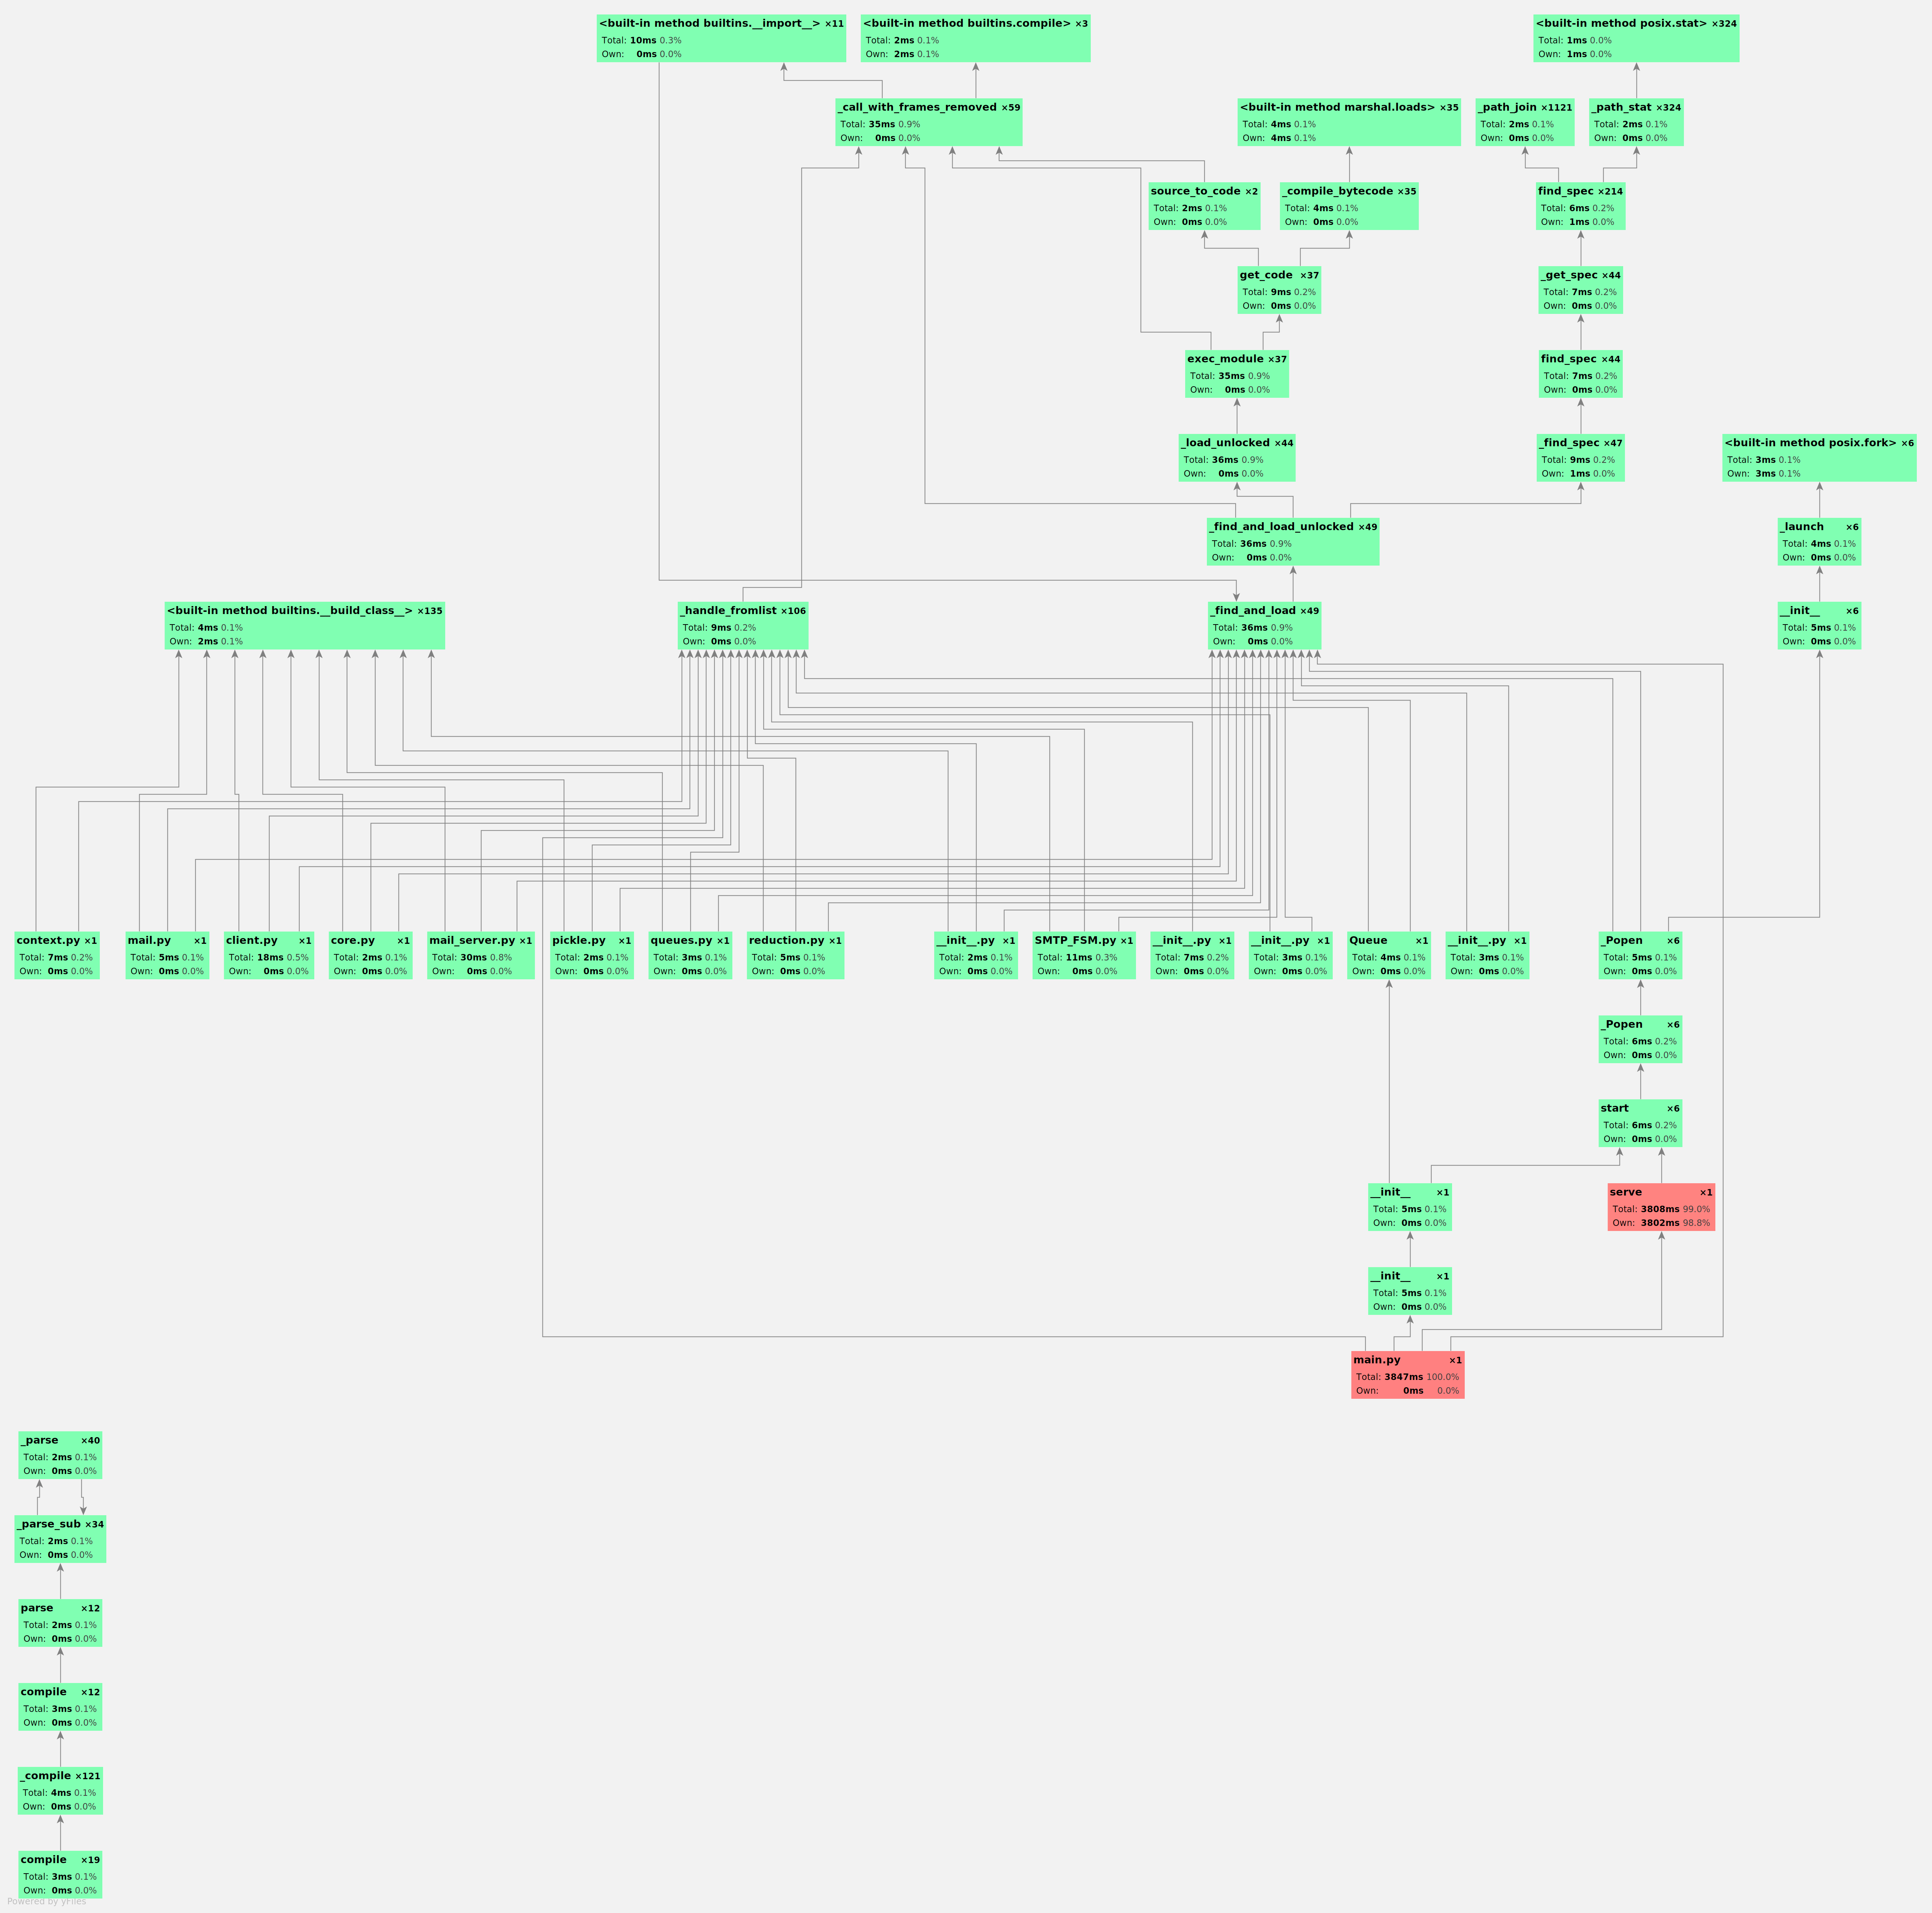
\includegraphics[width=\textwidth]{static/smtp-course-work14.png}
\caption{Граф вызовов}
\label{fig:cflow01}
\end{figure}

\vspace{100mm}

\section{Тестирование}

Ниже приведён отчет о модульном тестировании.

\begin{verbatim}

Launching pytest with arguments /home/v/programming/c/smtp-course-work in /home/v/programming/c/smtp-course-work

============================= test session starts ==============================
platform linux -- Python 3.7.5, pytest-5.3.2, py-1.8.0, pluggy-0.13.1 -- /home/v/programming/c/smtp-course-work/venv/bin/python
cachedir: .pytest_cache
rootdir: /home/v/programming/c/smtp-course-work
plugins: cov-2.8.1
collecting ... collected 13 items

server/tests/test_code.py::test_connection_to_server 
server/tests/test_code.py::test_send_mail_return 
server/tests/test_integr.py::test_send_simple_message_smtplib 
server/tests/test_integr.py::test_send_simple_message_socket 
server/tests/test_integr.py::test_send_message_two_recepients 
server/tests/test_maildir.py::test_maildir_duplicate 
server/tests/test_maildir.py::test_maildir_oversize 
server/tests/test_re.py::test_hello_pattern 
server/tests/test_re.py::test_email_pattern 
server/tests/test_re.py::test_email_patternf 
server/tests/test_re.py::test_data_end_patternf 
server/tests/test_re.py::test_data_end_patternf_should_match 
server/tests/test_sock.py::test_send_simple_message_socket 

============================== 13 passed in 2.50s==============================

\end{verbatim}
\addcontentsline{toc}{chapter}{Выводы}
\chapter*{Выводы}

В рамках предложенной работы нами был реализован SMTP-сервер в соответствии со стандартами RFC. В ходе работы реализованы следующие задачи: \\
\begin{enumerate}
	\item Проанализировали архитектурное решение
    \item Разработали подход для обработки входящих соединений и хранения входящих писем в maildir
    \item Рассмотрели \textbf{SMTP}-протокол
    \item Реализовали программу для получения писем по протоколу \textbf{SMTP}
    \item Рассмотрели работу с неблокирующими сокетами и их взаимодействие 
    \item Реализовали метод журналирования в отдельном процессе\textbf{SMTP}
    \item Разработали систему работающую в многозадачном режиме
    \item Познакомились с утилитами автоматической сборки и тестирования
\end{enumerate}
В ходе работы получены следующие навыки: \\
\begin{enumerate}
\item проектирования реализации сетевого протокола по имеющейся спецификации;
\item реализации сетевых приложений на языке программирования;
\item реализации сетевой службы без создания нити на каждое соединение;
\item автоматизированного системного тестирования ПО сетевой службы;
\item групповой работы с использованием системы контроля версий;
\end{enumerate}


\end{document}
